\appendix
\renewcommand{\chaptername}{Appendix}
\chapter{Decision Log}
\label{app:decisions}
Every place where the RiskSEA paper was silent or ambiguous, and every deviation, was logged when it was made. Values live in a configuration file, never in code.
{\footnotesize\singlespacing
\begin{longtable}{p{0.7cm} p{2.1cm} p{3.2cm} p{4.2cm} p{3.6cm}}
\toprule
\# & Topic & Paper says & Our choice & Reason\\
\midrule
\endhead
D1 & Behavioral feature list & References "Table 1" for features, but Table I is the data-source table. Says features are based on timestamp, amount, frequency of in/out transactions, for ETH and ERC-20 separately & Own list: amount stats, time stats, frequency, counterparties, in/out ratios, per ETH and ERC-20 & Matches the paper's textual description\\[2pt]
D2 & Embedding dimension & Not stated & 128 & node2vec default\\[2pt]
D3 & Skip-gram window / negatives / epochs & Not stated & window 10, negative 5, epochs 1 & gensim-typical defaults\\[2pt]
D4 & Propagation aggregation & "Aggregated embeddings of 5 sampled one-hop core neighbours" & Mean & Simplest, order-invariant\\[2pt]
D5 & Random forest & Not stated beyond "random forest" & 500 trees, class\_weight balanced & Standard, robust to imbalance\\[2pt]
D6 & Train/test split & Not stated & 80/20 stratified by address, fixed seeds, 5 seeds & Standard\\[2pt]
D7 & Decision threshold for P/R/F1 & Not stated & 0.5, plus PR-AUC and ROC-AUC reported & Threshold-free metrics avoid dependence\\[2pt]
D8 & Incremental step size & "Daily" training, but 10M->16M blocks at daily steps is \textasciitilde{}830 runs & \texttt{dynamic.step\_\allowbreak{}blocks} config (default 100K blocks), ablated & Almost certainly coarser in practice\\[2pt]
D9 & Edge definition & Directed; transactions between addresses & Directed, weight = interaction count (ETH + ERC-20) & Top-K ranking uses interaction count\\[2pt]
D10 & Table III / Figs 8-9 inconsistencies & Blank cells; p/q captions appear swapped & Run the full grid ourselves, do not trust captions & Cross-check\\[2pt]
D11 & Labels & Private (Coinbase internal + undisclosed external) & Public sources (to be assembled in M3) & Biggest deviation; judged by claims, not absolute numbers\\[2pt]
D12 & Development data & n/a & Synthetic world with planted fraud clusters (M1) before real data & Fast, deterministic debugging; real-data results are what count for the reproduction\\[2pt]
D13 & Walk direction & "Directed edges correspond to transactions" & Walks run over the undirected view (neighbors = in + out); \texttt{directed=True} available in \texttt{build\_\allowbreak{}graph} & A pure out-edge walk gets stuck at sinks (fraud collectors, cold wallets); propagation also uses "directly transacted" in either direction\\[2pt]
D14 & Walk edge weights & Top-K neighbors are chosen by interaction count; walk bias not specified & Weighted walks (probability proportional to interaction count x p/q factor) & Reference node2vec semantics; ablatable via \texttt{weighted} flag\\[2pt]
D15 & Distributed walk fidelity & "MapReduce split-apply-combine" & Per-walk uniforms taken from the same PCG64 stream as the in-memory generator, so the partitioned output is bit-identical (tested) & Proves distribution changes nothing about the algorithm\\[2pt]
D16 & Propagation vs dynamic training graph & Both "at similar checkpoints" & Propagation: node2vec on the \emph{induced subgraph of the core set} then one-hop propagation over the full graph; Dynamic: all addresses, incremental & Matches the paper's description of each method\\[2pt]
D17 & ERC-20 amounts & Not specified & Raw token units (decimals differ per token), plus distinct-token count; ETH value in ETH & Normalising needs a decimals table; revisit if ERC-20 features look unstable\\[2pt]
D18 & Extraction method & Not specified & Server-side aggregation in BigQuery with partition-pruning on block\_timestamp plus an exact block\_number cut; internal traces excluded & Avoids moving billions of raw rows; matches "transactions" and "ERC-20 transactions"\\[2pt]
D19 & eth-labels as a label source & n/a & \texttt{phish-hack} (bad) and \texttt{exchange} (good) files from dawsbot/eth-labels (MIT repo) used for development & The repo's data is scraped from Etherscan, whose terms of use are unclear; flagged to the user, who approved the download. Re-check before publishing results or redistributing the data\\[2pt]
D20 & Are labeled addresses in the core set? & "included all the addresses ... which have transacted with any addresses in the training set" (ambiguous) & Both variants are run: A) labeled addresses are core members (embeddings trained directly); B) labeled addresses are excluded from the core and only get propagated embeddings. Variant B is the faithful test of propagation & Cheap to run both; they answer different questions and the comparison is informative\\[2pt]
D21 & Heavy-tailed behavioral amounts & Not discussed & Behavioral features go through a monotone \texttt{sign(x)*log1p(|x|)} before the classifier & ERC-20 amounts are raw token units and in/out value ratios reach >1e38, overflowing float32 in the random forest; trees depend only on value ordering, so no information is lost\\[2pt]
D22 & Snapshots for Table IV & Daily-updated graph; edge counts per time step not specified & Time-sliced snapshots from each pair's first block, unweighted (exact counts per checkpoint are not in the extracted tables); each node keeps its top-200 neighbors by total count, then edges are filtered by first block & Edge existence never looks ahead; only the choice of which neighbors to keep uses final counts\\[2pt]
D23 & Table IV setup & Checkpoints 5M, 8M, 10M, 16M blocks; 30M-address core of 266M & Universe of 3M nodes around the labeled addresses, propagation core of 1M (labeled excluded), checkpoints 4.0M, 4.5M, 5.0M with an update every 250K blocks, configuration (10,10,1,1) throughout & Bad labels are scarce before 4M blocks (36 present at 4.0M); a 3M universe fits in 15.7 GiB at dimension 128; the core must be large enough to contain the labeled addresses' neighbors\\[2pt]
D24 & Table III protocol & Sweep on a 30M-address subsample; metric called AUC & Sweep on the 2.5M-node core subgraph, node2vec-only random-forest PR-AUC (area under the precision-recall curve), identical splits for all runs, and 3 extra training seeds of the base configuration to measure retraining noise & Differences in the paper are as small as 0.002, so noise had to be measured; PR-AUC is the paper's stated evaluation metric family\\[2pt]
\bottomrule
\end{longtable}
}

\chapter{Complete List of Deposit Addresses Found}
\label{app:deposits}
These are the 29 addresses on the phishing trace that the sweep rule classified as deposit addresses of the labeled exchange wallet \emph{ShapeShift 3}, ranked by share of the funds. They are inferred, medium-confidence results and a lead to be confirmed by the exchange, not proof. Shares sum to 90.9\% of the traced funds.
\gentable{gen/tab_deposits.tex}{The 29 inferred ShapeShift 3 deposit addresses (TTR-lite, phishing case).}{tab:deposits}

\chapter{Reproducibility and Commands}
\label{app:repro}
\section{Environment}
Windows 11, 16 cores, 15.7\,GiB RAM, Python 3.12; main libraries NumPy, pandas, DuckDB, scikit-learn, gensim 4.4, Numba, PyArrow, FastAPI and Uvicorn; Node.js 24 with Vite and React for the interface. This report and the comparative study were typeset with Tectonic. Raw data, graphs and embeddings are not under version control (large, regenerable, and some label sources have unclear terms of use).

\section{Reproduction pipeline order}
All scripts are in \code{scripts/}, tests in \code{tests/}.
\begin{enumerate}[label=\arabic*.]
\item \code{bq\_dry\_run.py}, \code{extract\_bq.py}, \code{download\_result.py}: dry-run costs, then extract and download the BigQuery tables (parallel, resumable, billing-capped).
\item \code{label\_overlap.py}, \code{real\_features.py}: label audit and behavioural features for labeled addresses.
\item \code{train\_core.py}: core selection and node2vec training (\code{--exclude-seeds} for variant B); \code{table2\_real.py}: Table~II.
\item \code{build\_snapshots.py}, \code{table4\_run.py}, \code{table4\_eval.py}: time-sliced adjacency, propagation and dynamic runs, Table~IV.
\item \code{sweep\_table3.py}, \code{sweep\_report.py}: Table~III sweep and its figures.
\item \code{tsne\_figures.py}, \code{make\_report\_tables.py}: t-SNE figures and every table of the comparative study, generated from result files.
\end{enumerate}

\section{Running CryptoTrace}
From the repository root, in PowerShell. The built interface in \code{frontend/dist} is served by the same process.
\begin{verbatim}
cd frontend; npm install; npm run build; cd ..
.\.venv\Scripts\python.exe -m uvicorn cryptotrace.api:app --app-dir src --port 8000
\end{verbatim}
Then open \url{http://127.0.0.1:8000}. For live tracing of any wallet (billed and capped), authenticate with \code{gcloud auth application-default login} and set \code{CRYPTOTRACE\_BQ\_PROJECT} before starting the server. To regenerate the cached benchmark results: \code{scripts\textbackslash ct\_run\_cases.py <project>}. To retake every screenshot of this report: \code{node scripts/ct\_screenshots.mjs <output-folder>} with the server running. Tests: \code{.\textbackslash.venv\textbackslash Scripts\textbackslash python.exe -m pytest -q} (78 tests).

\section{Repository history}
The work is on three commits on the branch used for the prototype: the initial reproduction pipeline, the addition of the sweep, t-SNE figures, the comparative LaTeX report and decision log entries D22--D24, and the polished tracing demo. All commits were made by the authors.

\chapter{Additional Figures}
\label{app:figs}
\begin{figure}[H]
\centering
\begin{subfigure}{0.48\textwidth}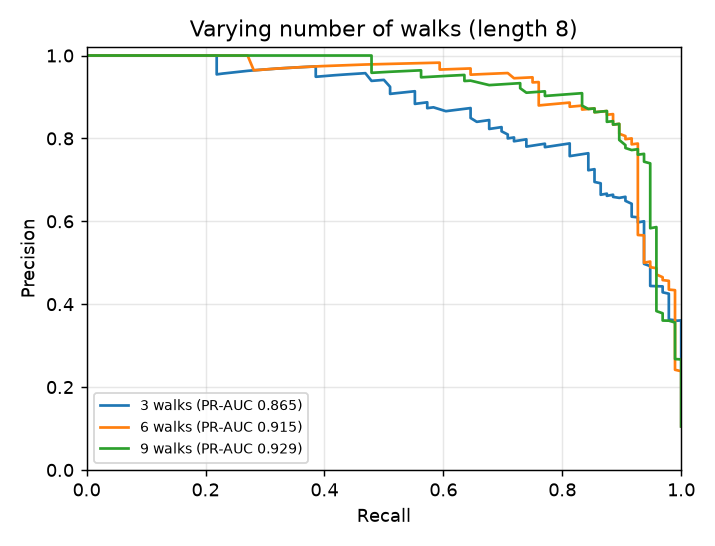
\includegraphics[width=\textwidth]{figures/sweep_fig5_walks}\caption{Number of walks.}\end{subfigure}\hfill
\begin{subfigure}{0.48\textwidth}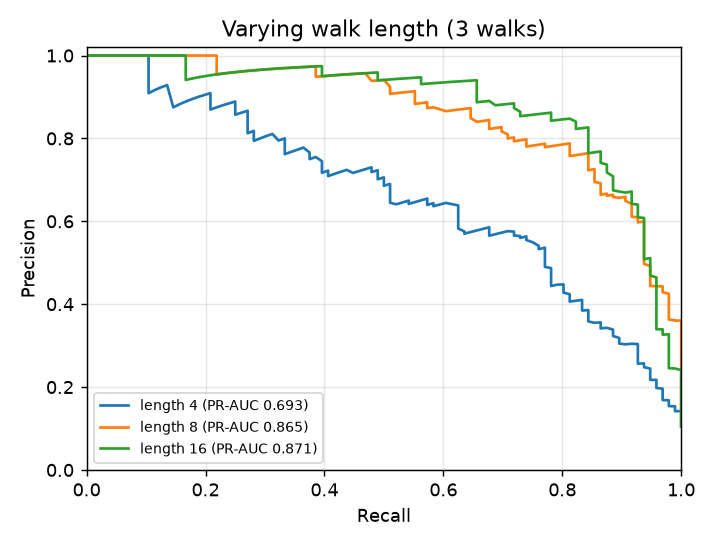
\includegraphics[width=\textwidth]{figures/sweep_fig6_length}\caption{Walk length.}\end{subfigure}\\[4pt]
\begin{subfigure}{0.48\textwidth}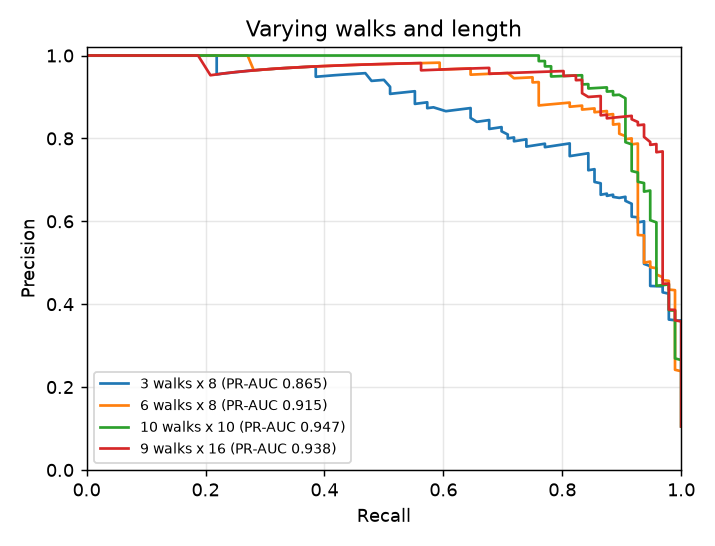
\includegraphics[width=\textwidth]{figures/sweep_fig7_joint}\caption{Walks and length.}\end{subfigure}\hfill
\begin{subfigure}{0.48\textwidth}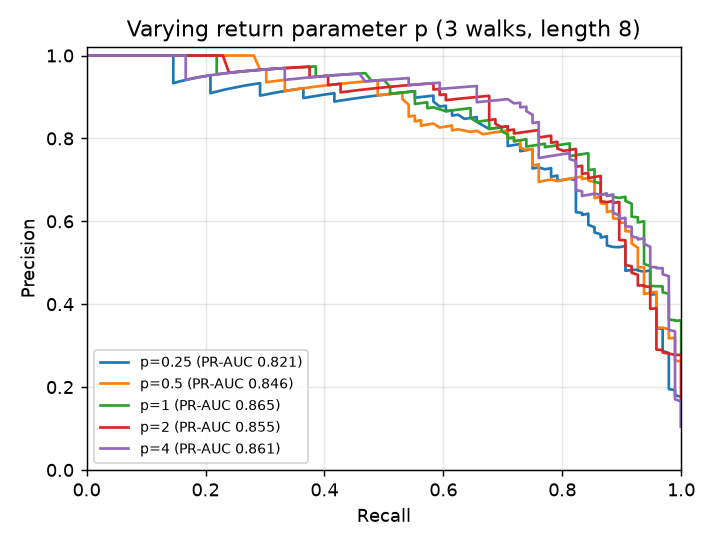
\includegraphics[width=\textwidth]{figures/sweep_fig8_p}\caption{Return parameter $p$.}\end{subfigure}\\[4pt]
\begin{subfigure}{0.48\textwidth}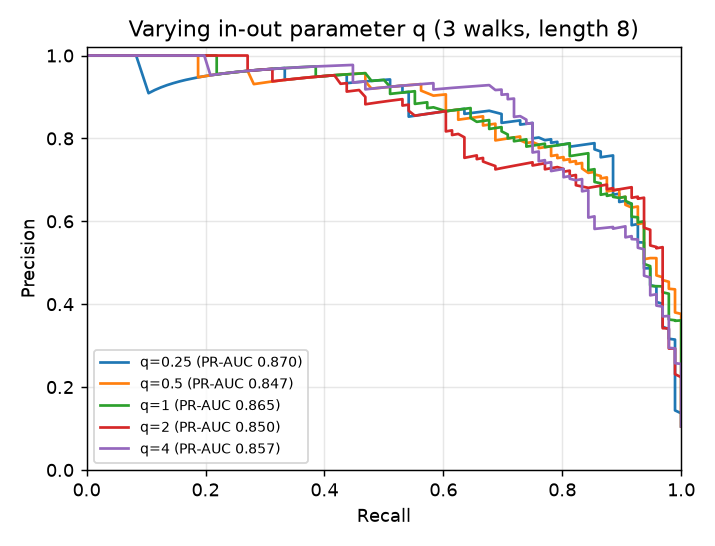
\includegraphics[width=\textwidth]{figures/sweep_fig9_q}\caption{In-out parameter $q$.}\end{subfigure}
\caption{Precision--recall curves of the Table~III sweep (analogs of the paper's Figures~5--9; one curve per setting from the first test split, legends give the mean PR-AUC over five splits).}
\label{fig:sweepcurves}
\end{figure}

\chapter{Full-Page Screenshots}
\label{app:screens}
The following captures show each page of the application at full length.
\shot{02_overview_full}{Overview page, full length.}
\shot{04_system_full}{System page, full length, with the planned modules shown.}
\shot{39_compare_full}{Compare page (phishing case), full length, including the published 20-case table.}
\shotw{41_gaps_full_p1}{Gaps page, first half.}{0.78}
\shotw{41_gaps_full_p2}{Gaps page, second half: remaining gaps and the roadmap.}{0.78}
\shotw{43_report_full_p1}{Investigator report, first half.}{0.78}
\shotw{43_report_full_p2}{Investigator report, second half: evidence paths, laundering patterns, method and limits.}{0.78}

\chapter{Chronological Work Log}
\label{app:log}
This log lists, in order, what was done and observed during the project, including approvals and corrections. It complements Table~\ref{tab:workdone}.
\begin{enumerate}[label=\arabic*.]
\item \textbf{Paper review.} The RiskSEA paper was read; we assessed which parts could be implemented from its text and which depend on private data (labels) or cluster scale.
\item \textbf{Plan.} An end-to-end reproduction workflow was written for execution step by step, with the instruction that every deviation be recorded; a first synthetic world with planted fraud clusters was used to debug before real data.
\item \textbf{Cost control first.} BigQuery dry runs were run before any extraction; the extraction was approved for a specific tier and cost; every query carried a billing cap equal to its dry run plus 5\%.
\item \textbf{Authentication.} Application-default credentials were set up by the user; the code base never handles credentials.
\item \textbf{Label sources.} Public sources were identified; the Etherscan-derived label lists and the OFAC list were downloaded only after explicit approval of each file, and the terms-of-use caveat was recorded (decision D19).
\item \textbf{Extraction and download.} The fast download path was blocked by policy, so parallel resumable REST reads were used; the highest block received was verified to be exactly 5\,000\,000.
\item \textbf{Graph, features, embeddings.} The staged DuckDB graph build replaced a first attempt that ran out of memory; features were log-compressed after a float32 overflow; the gensim integer-token trap was found and fixed.
\item \textbf{Experiments.} Table~II was run in two variants; the has-embedding leak was found and controlled; the Table~III sweep was run on the core subgraph with retraining noise measured; Table~IV was run at three checkpoints; t-SNE figures and cluster metrics were produced.
\item \textbf{Version control.} The user created the repository and made all commits; the assistant supplied commands only.
\item \textbf{Comparative study.} A LaTeX report compared the paper with the reproduction, starting with a comparison of data constraints; its PDF was produced.
\item \textbf{Extension study.} The textbook was read; RiskSEA was judged a strong baseline for scoring and infrastructure but not for tracing and attribution; eight research gaps were written in plain words and the architecture was sketched.
\item \textbf{CryptoTrace build.} Engines, providers, label store, API and interface were built; a dry run of the per-hop query gave 1.2\,GiB; validation on KuCoin and Cryptopia followed (Tornado Cash reached; EtherDelta reached; Yobit.net and OKEx not reached).
\item \textbf{Defects.} The dry-run placeholder, the provider time filter, the parent--child ping-pong, the exploration query over our own cap and several interface bugs were found and fixed (Table~\ref{tab:bugs}).
\item \textbf{Third case.} A real phishing-labeled wallet was found with an exploration query of 29.9\,GiB, traced for 19.9\,GiB, and added as the main demonstration case, with the selection bias disclosed.
\item \textbf{Polish.} Findings were grouped by receiving entity, a demo guide, keyboard shortcuts, automatic highlighting of the top finding, and a responsive layout were added; 78 tests pass.
\item \textbf{Presentation material.} Plain-language explanations of each screen and of the improvements over the baseline were prepared for the project presentation.
\item \textbf{This report.} Screenshots taken earlier were found to mismatch their file names in several cases (wrong strategy or case), so the screenshot script was rewritten and every screen was retaken before they were included.
\end{enumerate}
